\subsection{Construction and deletion results}
\label{app:root-robustness}
These checks reuse the frozen selections and 100 bps utility after the original outcomes were inspected. They neither add independent roots nor extend the original confirmatory family. Each method resamples the complete root vector across both regimes and all 24 estimands.

\begin{table}[h]\centering\small
\begin{tabular}{llrrr}\toprule
Regime & $\rho$ & LOO mean range & Max. LOO upper & Max. alternative upper\\\midrule
Liquid & 0 & [-13.26, -11.49] & -4.98 & -3.13\\
Liquid & 1 & [-13.50, -11.78] & -5.30 & -3.62\\
Thin & 0 & [-23.01, -21.83] & -15.28 & -15.61\\
Thin & 1 & [-22.63, -21.47] & -14.92 & -15.25\\
\bottomrule\end{tabular}
\caption{Largest scale $s=0.30$: all values are bps. Leave-one-root-out (LOO) checks refit a 24-estimate unstandardized maximum-deviation band using 49 shared roots and 20,000 draws for each of 50 deletions. Alternative bounds use two independently seeded paired-root runs, a fixed-sample-SE standardized paired-root maximum, and a standardized Gaussian root-multiplier maximum, each with 20,000 draws. No joint coverage is claimed across methods or deletions.}\label{tab:root-robustness}\end{table}

Standardization divides bootstrap deviations by the original sample standard error, not a reestimated standard error in each draw. Gaussian multipliers approximate the centered root-mean distribution using its empirical covariance. Constant observed columns are flagged; a zero empirical standard error does not establish zero population uncertainty. Numerical bands remain approximate and conditional on the frozen synthetic world.

\begin{figure}[h]\centering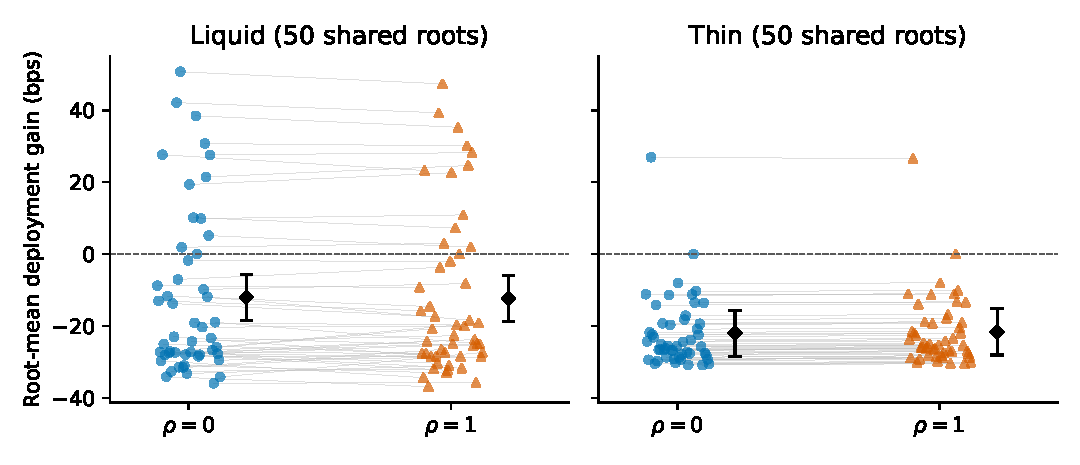
\includegraphics[width=.95\linewidth]{market_root_distribution.pdf}
\caption{Fifty root-level procedure gains at the largest scale under the original 100 bps utility. Each point averages four paired deployments; lines connect the same root across response settings. Incumbent-retaining roots contribute zero. Diamonds and bars show the original full-cohort means and 24-estimate simultaneous bands, not uncertainty for individual roots.}\label{fig:root-distribution}\end{figure}
